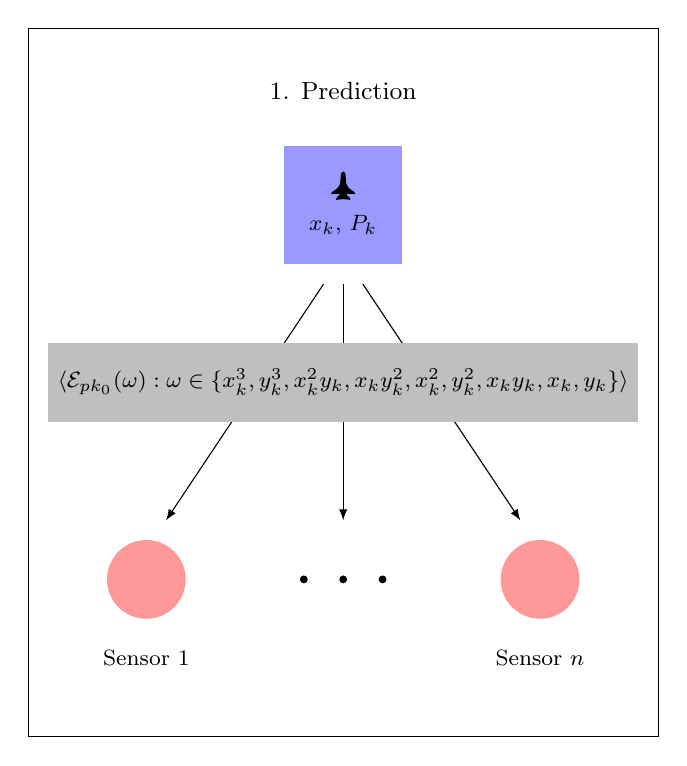
\begin{tikzpicture}[font=\footnotesize]

\draw  (0,0) rectangle (8,9);

\fill  [blue!40] (3.25, 7.5) rectangle (4.75, 6);
\node at (4,8.2) {\small 1. Prediction};

% Navigator
    \begin{scope}[shift={(4,7.1725)},xscale=0.22,yscale=0.3]
        % Plane
        \draw[fill]  plot[smooth, tension=.6] coordinates {
        (-0.65,-0.9) 
        (-0.6,-0.85) 
        (-0.4,-0.75) 
        (-0.25,-0.65) 
        (-0.15,-0.5) 
        (-0.12,-0.3) 
        (-0.10,-0.1) 
        (0.0,0.0) 
        (0.10,-0.1) 
        (0.12,-0.3) 
        (0.15,-0.5) 
        (0.25,-0.65) 
        (0.4,-0.75) 
        (0.6,-0.85) 
        (0.65,-0.9)
        } -- plot[smooth, tension=.6] coordinates {
        (0.65,-0.9) 
        (0.15,-0.91)
        (0.35,-1.1) 
        (0.37,-1.15)
        } -- plot[smooth, tension=.6] coordinates {
        (0.37,-1.15)
        (0.0,-1.12) 
        (-0.37,-1.15) 
        } -- plot[smooth, tension=.6] coordinates {
        (-0.37,-1.15)
        (-0.35,-1.1) 
        (-0.15,-0.91) 
        (-0.65,-0.9) 
        } -- cycle;
    \end{scope}
    
    \node at (4,6.5) {$x_k$, $P_k$};
    
    \fill  (1.5,2) [red!40] ellipse (0.5 and 0.5);
    \node at (1.5,1) {Sensor $1$};
    \fill  (6.5,2) [red!40] ellipse (0.5 and 0.5);
    \node at (6.5,1) {Sensor $n$};
    
    \fill [black] (3.5,2) circle (0.05);
    \fill [black] (4,2) circle (0.05);
    \fill [black] (4.5,2) circle (0.05);
    
    
	
	\draw [-latex] plot[smooth, tension=.7] coordinates {(3.75,5.75) (1.75,2.75)};
	\draw [-latex] plot[smooth, tension=.7] coordinates {(4.25,5.75) (6.25,2.75)};
	\draw [-latex] plot[smooth, tension=.7] coordinates {(4,5.75) (4,2.75)};
	
	
	\fill [lightgray]  (0.25,5) rectangle (7.75,4);
	\node at (4,4.5) {$\langle\mathcal{E}_{pk_0}(\omega): \omega \in \{x^3_k, y^3_k, x^2_ky_k, x_ky^2_k, x^2_k, y^2_k, x_ky_k, x_k, y_k\}\rangle$};
	

	

\end{tikzpicture}